\section{Introducción}

Luego de haber ayudado a Scaloni y el equipo técnico a no solo ordenar los análisis de los siguientes rivales sino también elegir el mejor cronograma de entrenamientos de la selección \textbf{CAMPEONA DEL MUNDO}, Scaloni comenzó a armar la plantilla para el mundial 2026 que traerá la $4ta$ a casa \textbf{(se anula todo tipo de mufa)}. A su vez, la prensa está metiendo presión y cada medio está dando su conjunto de jugadores que les gustaría ver jugar con la albiceleste. Ante esta presión, Scaloni se topó con el problema de querer encontrar la mínima cantidad de jugadores para contentar a todos. Con tener un jugador que contente a cada medio le es suficiente.
Como no podía ser de otra manera, el gran Bilardo, astuto pues ya se conoce todos los problemas con la prensa, le comenta que este no es más que un caso particular del $Hitting Set Problem$, el cual es:
\textit{Dado un conjunto $A$ de $n$ elementos y $m$ subconjuntos $B_1, B_2, ..., B_m$ de $A$ ($B_i \subseteq A \forall i$) , queremos el subconjunto $C \subseteq A$ de menor tamaño tal que $C$ tenga al menos un elemento de cada $B_i$ (es decir, $C \cap B_i \neq \emptyset$)}.
En nuestro caso, $A$ son los jugadores convocados, los $B_i$ son los deseos de la prensa, y $C$ es el conjunto de jugadores que deberían jugar si o si en la selección.
Scaloni solicita nuestra ayuda para ver si este subconjunto de jugadores se puede obtener eficientemente, es decir, en tiempo polinomial, o se nos complica obtener dicho subconjunto más de lo que se pretende.

Ahora bien, ¿Qué significa eso de \textit{''tiempo polinomial''}? ¿Existe algo peor? ¿A dónde puede llegar todo esto? Vamos de a poco.
En el mundo de la teoría de la complejidad computacional existe lo que se conoce como \textit{Clases de Complejidad}. Segun \href{https://es.wikipedia.org/wiki/Clase_de_complejidad}{Wikipedia}, la definicion es la siguiente:
\begin{quote}
En teoría de la complejidad computacional, una clase de complejidad es un conjunto de problemas de decisión de complejidad relacionada. Una clase de complejidad tiene una definición de la forma:

\textit{el conjunto de los problemas de decisión que pueden ser resueltos por una máquina M utilizando O(f(n)) del recurso R (donde n es el tamaño de la entrada)}.
\end{quote}

Existen diversas clases de complejidad, y aquí se enumeran algunas de ellas:
\begin{itemize}
	\item \texttt{P}: problemas que se resuelven en tiempo polinomial, es decir, son bastantes eficientes.
	\item \texttt{NP}: problemas que sus soluciones se pueden verificar en tiempo polinomial. Con esto podemos afirmar que todo problema que está en P, también está en NP, ya que si encontramos la solución en tiempo polinomial, también la podremos validar en tiempo polinomial\footnote{Aclarar que no vale su inversa, ya que no todo problema de $NP$ se encuentra en $P$, por lo que $NP \not\subset  P$.}.
    \[ P \subset NP\]
	\item \texttt{NP-Completos}: problemas de decisión los cuales la respuesta pueden ser ''si'' o ''no'' dependiendo si se puede resolver el problema. Estos problemas son los más difíciles de los problemas que se pueden verificar su solución en tiempo polinomial, es decir, los más difíciles de los NP.
    Por lo tanto,
    \[ P \subset NP \subset NP-Completos\]
	\item \texttt{PSPACE}: problemas que para encontrar su solución se requiere un espacio polinomial de memoria.
\end{itemize}
Ahora bien, si hablamos de clases de complejidad y problemas NP-Completos, también debemos hablar de $Reducciones$. Según \href{https://es.wikipedia.org/wiki/Reducci%C3%B3n_(complejidad)}{Wikipedia}:
\begin{quote}
    En teoría de la computación y teoría de la complejidad computacional, una reducción es una transformación de un problema a otro problema. Dependiendo de la transformación usada, la reducción se puede utilizar para definir clases de complejidad en un conjunto de problemas.

    Intuitivamente, un problema $A$ es reducible a un problema $B$ si las soluciones de $B$ existen y dan una solución para $A$ siempre que $A$ tenga solución. Así, resolver $A$ no puede ser más difícil que resolver $B$. Normalmente, esto se expresa de la forma $A \leq B$, y se añade un subíndice en $\le$ para indicar el tipo de reducción utilizada. Por ejemplo, se usa la letra $p$ como subíndice para indicar que la reducción puede realizarse en tiempo polinomial: $A \leq _p B$
\end{quote}

En otras palabras, si reducimos un problema $A$ a un problema $B$, resolver el problema $A$ será como mucho tan difícil de resolver como el problema $B$. Esto va a ser de gran utilidad, ya que se ha demostrado distintos problemas que son \texttt{NP-Completos}, y muchas veces para poder demostrar esto se ha utilizado y se puede utilizar la propiedad de transitividad, que es que si tengo un problema $A$ tal que $A \in \texttt{NP-Completos}$, y un problema $B$ que desconozco su dificultad pero pertenece a $NP$, en caso que logre reducir $A$ a $B$, $B$ también es \texttt{NP-Completos}. Es decir

\[ A \in {NP-C}: A \leq _p B \Rightarrow B \in NP-C \]

\subsection{Hitting-Set Problem}

Volviendo al problema del Hitting-Set Problem, empecemos por ver si este pertenece a \texttt{NP}. Para ello, recordemos que los problemas pertenecientes a NP son aquellos los cuales se pueden verificar su solución en tiempo polinomial. Para este caso, $Hitting-Set Problem \in \texttt{NP}$ de la siguiente manera: dado un conjunto $C$ como solución al problema y un conjunto $A$ con todos los elementos, y subconjuntos $B_i$ tal que $\forall B_i: B_i \subseteq A$, es sencillo verificar que la solución es válida siguiendo los siguientes pasos: para cada $B_i$ verificar que al menos uno de sus elementos está en el conjunto $C$. En caso que haya un $B_i$ donde no esté ninguno de sus elementos en $C$, la solución no será válida. Por lo tanto, la complejidad para verificar la solución será $\mathcal{O}(n \times m)$ siendo $n$ la cantidad de subconjuntos $B$, y $m$ la cantidad de elementos de cada subconjunto. Por lo tanto, la verificación de la solución $\subset \texttt{P} \Rightarrow Hitting-Set Problem \in \texttt{NP}$.

Supongamos que tenemos el conjunto $A = (1, 2, 3, 4, 5, 6, 7, 8, 9, 10)$, y los subconjuntos $B = ((1, 2), (3, 4), (5, 6), (7, 8), (9, 10))$, y el conjunto solución $C = (1, 3, 6, 7)$. La verificación tendrá el siguiente formato:

\begin{lstlisting}[language=Python]
if len(C) > len(B): return false
for subconjunto in B:
    hay_un_elemento = false
    for elemento in subconjunto:
   	 if elemento in C:
   		 hay_un_elemento = true
    if not hay_un_elemento: return false
return true
\end{lstlisting}

La primera línea hace referencia a la validez de que es el conjunto mínimo que abarca todos al menos un elemento de todos los subconjuntos. Ya que si tengo N subconjuntos, la cantidad máxima que debo tener como solución debe ser N elementos (esto es así ya que el peor de los casos es que todos los subconjuntos no compartan ningún elemento).

Siguiendo con el ejemplo, la verificación devolverá false ya que no hay ningún elemento en el conjunto $C$ que representa el subconjunto $(9, 10)$.

Continuando con el problema del Hitting-Set, ¿Es posible que $Hitting-Set \in \texttt{NP-Completo}$?
Para que se cumpla eso, podemos aprovecharnos de la propiedad de transitividad y reducir polinomialmente un problema que sabemos que es \texttt{NP-Completo} a Hitting-Set. Ahora bien, tenemos que encontrar un problema el cual nos pueda facilitar esta transformación (siempre y cuando exista la posibilidad de que Hitting-Set sea NP-Completo).

Para ello, usaremos el problema del Dominating-Set (prueba que es \href{https://www.geeksforgeeks.org/proof-that-dominant-set-of-a-graph-is-np-complete/}{\texttt{NP-Completo}}). Dominating-Set es un problema el cual propone que dado un grafo G, encontrar el subconjunto $D$ de vértices de G tal que: $\forall v \in G: v \in D \lor w \in D$, siendo $w$ un adyacente a $v$, y este subconjunto el más chico posible. Ahora está la pregunta, ¿Cómo podemos hacer para transformar el grafo y el problema de Dominating-Set de tal manera que haciendo uso del Hitting-Set, devuelva si existe o no una solución al problema del Dominating-Set de tamaño como mucho $k$?

En el Hitting-Set, lo que nos condiciona es que para cada subconjunto, haya al menos un representante, y buscar el conjunto solución tal que sea mínimo. Por el otro lado, en el Dominating-Set lo que nos condiciona es el hecho de que si o si dado un vértice $v$ y sus adyacentes, al menos uno de dichos vértices deben estar en el subconjunto $D$. Esto ya nos va indicando cómo podemos hacer posible la reducción, dado que podemos empezar a ver cómo se pueden formar nuestros $B_i$ del Hitting-Set. Empecemos por lo básico: transformar el grafo.

Ya que con lo que debemos cumplir son los subconjuntos $B_i$ que haya al menos un elemento de cada uno, sería acorde que los vértices del grafo sean los elementos de todo el conjunto $A$. Falta lo importante y la parte clave: cómo relacionar estos vértices de manera que al pasar la transformación de nuestro grafo a nuestra ''caja negra'' que resuelve un Hitting-Set, nos devuelva que puede existir solución de como mucho $k$ elementos, siendo $k$ la cantidad de vértices del grafo original. La relacion sera de la siguiente manera:
\begin{itemize}
    \item Para cada vertice $v_i$, se creará un subconjunto $B_i$ el cual contendrá a $v_i$ y todos sus adyacentes, es decir, $\forall v_i \in G: \forall w_i \in adyacentes(v_i): v_i \in B_i \land w_i \in B_i$.
    \item Habrá tantos subconjuntos $B_i$ como vértices en el grafo, y el tamaño de estos subconjuntos será la cantidad de adyacentes que tenga el vértice a partir del cual se genero el subconjunto.
\end{itemize}

Por ejemplo para los siguientes grafos, les correspondera los siguientes subconjuntos:

\begin{figure}[H]
	\centering
	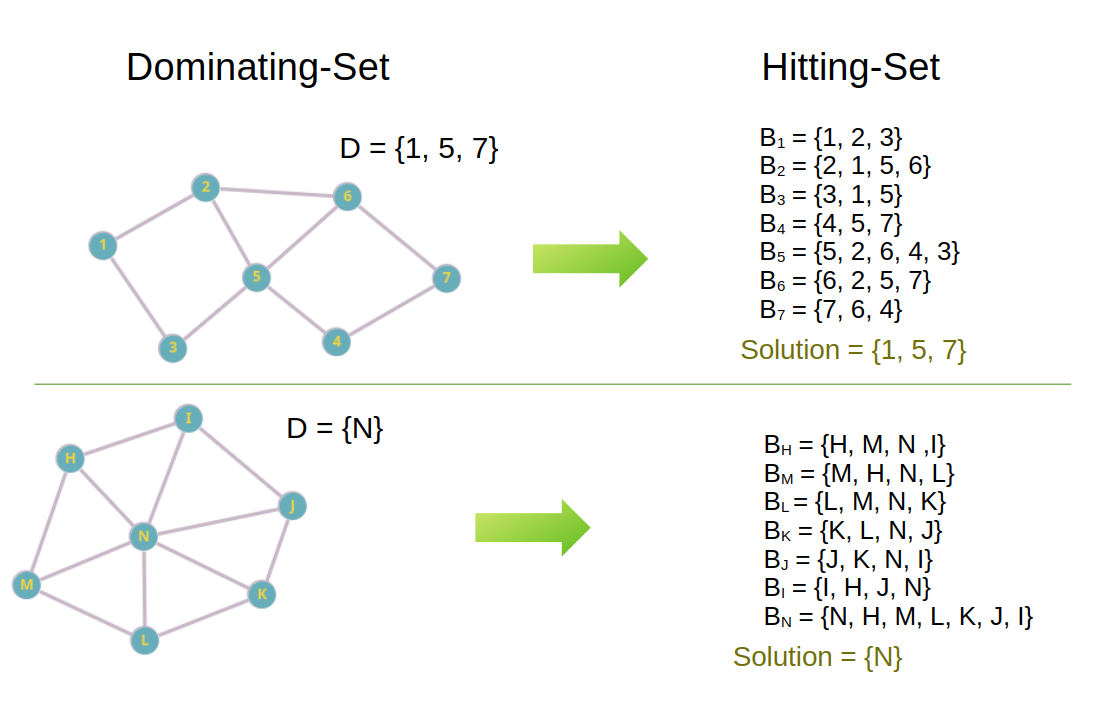
\includegraphics[width=0.9\textwidth]{img/dshs.png}
\end{figure}

De esta manera, una vez creados todos los subconjuntos $B_i$, al pasar a la ''caja negra'' que resuelve el Hitting-Set nuestro conjunto y un valor $k$, nos devolverá si existe o no una solución la cual contenga como mucho $k$ elementos, que ''interpretado'' a nuestro problema original del Dominating-Set, que existan como mucho $k$ vértices pertenecientes al conjunto $D$. Una vez obtenida la salida de nuestra ''caja negra'' que diga si existe o no una solución al problema, podría hacerse un estilo de \textit{Búsqueda Binaria} para encontrar el conjunto mínimo del Dominating-Set.

Al ser Dominating-Set un problema \texttt{NP-Completo}, por propiedad de la transitividad, queda demostrado que el $Hitting-Set \subset \texttt{NP-Completo}$.
